\chapter{Introduction}

\textbf{TODO: 1.15, 1.16, 1.20, 1.26, 1.27 + CALCULUS OF VARIATIONS: 1.25, 1.34}

\section*{Exercise 1.1 $\star$}
Consider the sum-of-squares error function given by (1.2) in 
which the function $y(x, \mathbf{w})$ is given by the polynomial
(1.1). Show that the coefficients $\mathbf{w} = \{ w_i \}$ that minimize
this error function are given by the solution to the following
set of linear equations
\begin{equation}\label{eq:1.122}\tag{1.122}
    \sum_{j=0}^{M} A_{ij}w_j = T_i
\end{equation}
where 
\begin{equation}\label{eq:1.123}\tag{1.123}
    A_{ij} = \sum_{n=1}^{N} (x_n)^{i + j}, \hspace{5em} T_i = \sum_{n=1}^{N} (x_n)^it_n.
\end{equation}
Here a suffix $i$ or $j$ denotes the index of a component, whereas
$(x)^i$ denotes $x$ raised to the power of $i$.

\vspace{1em}

\begin{proof}
    The function $y(x, \mathbf{w})$ is given by
    \begin{equation*}\label{eq:1.1}\tag{1.1}
        y(x, \mathbf{w}) = \sum_{j = 0}^M w_j x^j
    \end{equation*}
    and the error function is given by
    \begin{equation*}\label{eq:1.2}\tag{1.2}
        E(\mathbf{w}) = \frac{1}{2} \sum_{n = 1}^N \{y(x_n, \mathbf{w}) - t_n\}^2
    \end{equation*}

    Since we want to find the coefficients $\mathbf{w}$ for which
    the error function is minimized, we compute its derivative with
    respect to $\mathbf{w}$:
    \begin{align*}
        \dv{\mathbf{w}} E(\mathbf{w}) 
        =& \dv{\mathbf{w}} \bigg(\frac{1}{2} \sum_{n = 1}^N \{y(x_n, \mathbf{w}) - t_n\}^2\bigg)
        = \frac{1}{2} \sum_{n = 1}^{N} \dv{\mathbf{w}} \{y(x_n, \mathbf{w})^2 - 2t_ny(x_n, \mathbf{w}) + t_n^2\} \\
        =& \sum_{n = 1}^N y(x_n, \mathbf{w}) \dv{\mathbf{w}} y(x_n, \mathbf{w})
            - \sum_{n = 1}^N t_n \dv{\mathbf{w}} y(x_n, \mathbf{w}) \label{eq:1.1.1}\tag{1.1.1}
    \end{align*}

    We continue by computing the derivative of $y(x_n, \mathbf{w})$ separately and obtain that:
    \begin{equation}\label{eq:1.1.2}\tag{1.1.2}
        \dv{\mathbf{w}} y(x_n, \mathbf{w}) 
        = \begin{bmatrix}
            x_n^1 \\
            \vdots \\
            x_n^M
        \end{bmatrix}
    \end{equation}

    By substituting the result of ($\ref{eq:1.1.2}$) into ($\ref{eq:1.1.1}$) we get that:
    \begin{equation}\label{eq:1.1.3}\tag{1.1.3}
        \dv{\mathbf{w}} E(\mathbf{w}) = B - T
    \end{equation}
    where $T$ is given by (\ref{eq:1.123}) and
    \[
        B_i = \sum_{n = 1}^{N} x_n^i y(x_n, \mathbf{w})  
    \] 

    Now, we easily find that
    \[
        B_i = \sum_{n = 1}^{N} \bigg(x_n^i \sum_{j = 0}^M w_j x_n^j\bigg)
        = \sum_{n = 1}^{N} \sum_{j = 0}^M x_n^{i + j} w_j
        = A_i \mathbf{w}
    \] 
    where $A$ is given by ($\ref{eq:1.123}$). Now, the critical point of $E(\mathbf{w})$ 
    is given by the equation:
    \[
        A_i \mathbf{w} = T_i
    \] 
    which is equivalent with $(\ref{eq:1.122})$.
\end{proof}

\section*{Exercise 1.2 $\star$}
Write down the set of coupled linear equations, analogous to (\ref{eq:1.122}), satisfied
by the coefficients $w_i$ which minimize the regularized sum-of-squares error
function given by ($\ref{eq:1.4}$).
    
\vspace{1em}

\begin{proof}
    The regularized sum-of-squares error function is given by
    \begin{equation}\label{eq:1.4}\tag{1.4}
        \widetilde{E}(\mathbf{w}) = \frac{1}{2} \sum_{i = 1}^N 
            \{y(x_n, \mathbf{w}) - t_n\}^2 + \frac{\lambda}{2} ||\mathbf{w}||^2
    \end{equation}

    We'll have a similar approach to the previous exercise, i.e. we compute
    the derivative of the regularized error function and find the associated
    critical point. We notice that
    \[
        \widetilde{E}(\mathbf{w}) = E(\mathbf{w}) + \frac{\lambda}{2} ||\mathbf{w}||^2
    \] 
    so
    \[
        \dv{\mathbf{w}} \widetilde{E}(\mathbf{w}) 
        = \dv{\mathbf{w}} E(\mathbf{w}) + \frac{\lambda}{2} \cdot \dv{\mathbf{w}} ||\mathbf{w}||^2
    \] 

    One could easily prove that
    \[
        \dv{\mathbf{w}} ||\mathbf{w}||^2 = 2\mathbf{w}
    \] 
    so by using this and $(\ref{eq:1.1.3})$ (where we substitute $B = A\mathbf{w}$), we
    have that:
    \[
        \dv{\mathbf{w}} \widetilde{E}(\mathbf{w}) 
        = A\mathbf{w} + \lambda \mathbf{w} - T
        = (A + \lambda I)\mathbf{w} - T
    \] 

    We obtain the critical point when the derivative is 0, so when
    \[
        (A + \lambda I) \mathbf{w} = T
    \] 
    which is equivalent with the system of linear equations
    \[
        \sum_{j=0}^{M} C_{ij} w_j = T_i
    \] 
    where 
    \[
        C_{ij} = A_{ij} + \lambda I_{ij} \hspace{2em}
    \] 
\end{proof}

\section*{Exercise 1.3 $\star \star$}
Suppose that we have three coloured boxes $r$ (red), $b$ (blue), and $g$ (green). Box
$r$ contains 3 apples, 4 oranges and 3 limes, box $b$ contains 1 apple, 1 orange, and 0
limes, and box $g$ contains 3 apples, 3 oranges, and 4 limes. If a box is chosen
at random with probabilities $p(r) = 0.2$, $p(b) = 0.2$, $p(g) = 0.6$, and a picee 
of fruit is removed from the box (with equal probability of selecting any of the items
in the box), then what is the probability of selecting an apple? If we observe
that the selected fruit is in fact an orange, what is the probability that it came from
the green box?

\vspace{1em}

\begin{proof}
    The conditional probabilities of obtaining a fruit knowing that we are 
    searching in a certain box are easily found since the fruits are equally
    likely to be extracted. We also now the probabilities of choosing a specific box,
    so we can simply apply the sum rule to obtain the probability of getting an apple:
    \[
        p(\text{apple}) 
        = p(\text{apple} | r)p(r) + p(\text{apple} | b)p(b) + p(\text{apple} | g)p(g) 
        = \frac{3}{10} \cdot 0.2 + \frac{1}{2} \cdot 0.2 + \frac{3}{10} \cdot 0.6
        = 34\%
    \] 

    If we know the selected fruit is an orange, the probability that it came from
    the green box is given by the Bayes' theorem:

    \begin{equation*}\label{eq:1.3.1}\tag{1.3.1}
        p(g | \text{orange}) = \frac{p(g)p(\text{orange} | g)}{p(\text{orange})}
    \end{equation*}

    The probability of choosing the green box is known and the probability of getting
    an orange from the green box is also easily found. We only need to find the probability
    of extracting an orange in the general case:
    \[
        p(\text{orange}) 
        = p(\text{orange} | r)p(r) + p(\text{orange} | b)p(b) + p(\text{orange} | g)p(g) 
        = \frac{4}{10} \cdot 0.2 + \frac{1}{2} \cdot 0.2 + \frac{3}{10} \cdot 0.6
        = 36\%
    \]

    The needed probability is now found by substituting the values in $(\ref{eq:1.3.1})$:
    \[
        p(g | \text{orange}) = \frac{0.6 \cdot \frac{3}{10}}{\frac{36}{100}} = \frac{1}{2} = 50\%
    \] 
\end{proof}

\section*{Exercise 1.4 $\star \star$}
Consider a probability density $p_x(x)$ defined over a continuous variable
$x$, and suppose that we make a nonlinear change of variable using $x = g(y)$,
so that the density transforms according to (1.27). By differentiating (1.27),
show that the location  $\widehat{y}$ of the maximum of the density in
$y$ is not in general related to the location $\widehat{x}$ of the maximum of the
density over $x$ by the simple functional relation $\widehat{x} = g(\widehat{y})$ 
as a consequence of the Jacobian factor. This shows that the maximum of a probability
density (in contrast to a simple function) is dependent of the choice of variable.
Verify that, in the case of a linear transformation, the location of the maximum
transforms in the same way as the variable itself.

\vspace{1em}

\begin{proof}
    If we make a nonlinear change of variable $x = g(y)$ in the probbability density 
    $p_x(x)$, it transforms according to
    \begin{equation}\label{eq:1.27}\tag{1.27}
        p_y(y) = p_x(g(y)) |g'(y)|
    \end{equation}

    We assume that the mode of $p_x(x)$ is given by an unique $\widehat{x}$, i.e.
     \[
         p_x'(x) = 0 \iff x = \widehat{x}
    \] 

    Now, let $s \in \{-1, 1\}$ such that $g'(y) = sg'(y)$. 
    The derivative of  $(\ref{eq:1.27})$ with respect to $y$ is given by:
    \[
        p_y'(y) = sp'x(g(y))\{g'(y)\}^2 + sp_x(g(y))g''(y)
    \] 

    For a linear change of variable, we have that $g''(y) = 0$, so the mode of $p_y(y)$ 
    is given by $g'(y) = 0$ and since $x = g(y)$, respectively $x' = g'(y)$ we have that
    $\widehat{x} = g(\widehat{y})$. Therefore, for a linear change of variable, the location
    of the maximum transforms in the same way as the variable itself.

    For a nonlinear change of variable, the second derivative will not be generally 0, so
    the mode is not given by $g'(y) = 0$ anymore. As a result, in general $\widehat{x} \neq g(\widehat{y})$,
    so the location of the mode will transform differently from the variable itself.
\end{proof}

\section*{Exercise 1.5 $\star$}
Using the definition ($\ref{eq:1.38}$) show that var$[f(x)]$ satisfies ($\ref{eq:1.39}$).

\vspace{1em}

\begin{proof}
    The variance is defined by 
    \begin{equation}\label{eq:1.38}\tag{1.38}
        \text{var}[f] = \mathbb{E}\big[(f(x) - \mathbb{E}[f(x)])^2\big]
    \end{equation}

    We expand the square and then use the linearity of expectation to obtain:
    \[
        \text{var}[f] 
        = \mathbb{E}\big[f(x)^2 - 2f(x)\mathbb{E}[f(x)] + \mathbb{E}[f(x)]^2\big]
        = \mathbb{E}[f(x)^2] - 2\mathbb{E}\big[f(x)\mathbb{E}[f(x)]\big] + \mathbb{E}\big[\mathbb{E}[f(x)]^2\big]
    \] 

    Since $\mathbb{E}[f(x)]$ is a constant, the expression of the variance becomes:
    \begin{equation}\label{eq:1.39}\tag{1.39}
        \text{var}[f] 
        = \mathbb{E}[f(x)^2] - 2\mathbb{E}[f(x)]^2 + \mathbb{E}[f(x)]^2
        = \mathbb{E}[f(x)^2] - \mathbb{E}[f(x)]^2
    \end{equation}
\end{proof}

\section*{Exercise 1.6 $\star$}
Show that if two variables $x$ and $y$ are independent, then their covariance is zero.

\vspace{1em}

\begin{proof}
    The covariance of two random variables is given by:
    \begin{equation}\label{eq:1.41}\tag{1.41}
        \text{cov}[x, y] = \mathbb{E}_{x, y} [xy] - E[x]E[y]
    \end{equation}

    We assume that the variables are continuous, but the discrete case result is similarly obtained.
    If $x$ and $y$ are independent, we have that $p(x, y) = p(x)p(y)$, so
     \[
         E_{x, y}[xy] = \iint p(x, y) xy \hspace{0.25em} \diff x \diff y 
         = \iint p(x) p(y) xy \hspace{0.25em} \diff x \diff y
         = \bigg(\int p(x) x \hspace{0.25em} \diff x\bigg) \bigg(\int p(y) y \hspace{0.25em} \diff y\bigg)
         = E[x]E[y]
    \] 
    and ($\ref{eq:1.41}$) becomes 0.
\end{proof}

\section*{Exercise 1.7 $\star \star$}
In this exercise, we prove the normalization condition (1.48) for the univariate
Gaussian. To do this consider the integral
\begin{equation}\label{eq:1.124}\tag{1.124}
    I = \int_{-\infty}^{\infty} \exp\bigg(-\frac{1}{2\sigma^2}x^2\bigg) \hspace{0.25em} \diff x
\end{equation}
which we can evaluate by first writing its square in the form
\begin{equation}\label{eq:1.125}\tag{1.125}
    I^2 = \int_{-\infty}^{\infty} \int_{-\infty}^{\infty} \exp 
        \bigg(-\frac{1}{2\sigma^2}x^2 - \frac{1}{2\sigma^2}y^2\bigg) \hspace{0.25em} \diff x\diff y
\end{equation}

Now make the transformation from Cartesian coordinates $(x, y)$ to polar coordinates $(r, \theta)$ 
and then substitute $u = r^2$. Show that, by performing the integrals over $\theta$ and $u$,
and then taking the square root of both sides, we obtain
\begin{equation}\label{eq:1.126}\tag{1.126}
    I = (2\pi\sigma^2)^{1/2}
\end{equation}

Finally, use this result to show that the Gaussian distribution $\mathcal{N}(x | \mu, \sigma^2)$ is 
normalized.

\vspace{1em}

\begin{proof}
    We transform $(\ref{eq:1.125})$ from Cartesian coordinates to polar coordinates and obtain:
\[
    I^2 = \int_{0}^{2\pi} \int_0^\infty \exp 
        \bigg(-\frac{r^2\sin^2 \theta + r^2\cos^2 \theta}{2\sigma^2}\bigg) r\diff r\diff \theta
        = \int_{0}^{2\pi} \int_{0}^{\infty} \exp \bigg(-\frac{r^2}{2\sigma^2}\bigg) r\diff r\diff \theta
    \] 

    We use the substitution $u = r^2$ and then compute the integral to get:
    \[
        I^2 = \frac{1}{2} \int_{0}^{2\pi} \int_{0}^{\infty} \exp\bigg(-\frac{u}{2\sigma^2}\bigg) du\diff \theta
        = \frac{1}{2} \int_0^{2\pi} -2\sigma^2 \exp\bigg(-\frac{u}{2\sigma^2}\bigg)\bigg|_0^\infty \diff \theta
        = \sigma^2 \int_{0}^{2\pi} \diff \theta = 2\pi\sigma^2
    \] 

    If we take the square root of this we see that
    \begin{equation}\tag{1.126}
        I = (2\pi\sigma^2)^{1/2}
    \end{equation}

    We can assume without loss of generality that the mean of the Gaussian is 0,
    as we could make the change of variable $y = x - \mu$. Therefore, by using
    $(\ref{eq:1.126})$ we obtain
    \[
        \mathcal{N}(x | \mu, \sigma^2) 
        = \frac{1}{\sqrt{2\pi\sigma^2}} \int_{-\infty}^{\infty} \exp\bigg(-\frac{x}{2\sigma^2}\bigg) \diff x
        = \frac{I}{\sqrt{2\pi\sigma^2}} = 1
    \] 
    which shows that the Gaussian distribution is normailized.
\end{proof}

\section*{Exercise 1.8 $\star \star$}
By using a change of variables, verify that the univariate Gaussian
given by (1.46) satisfies ($\ref{eq:1.49}$). Next, by differentiating both sides
of the normalization condition
\begin{equation*}\label{eq:1.127}\tag{1.127}
    \int_{-\infty}^{\infty} \mathcal{N} (x | \mu, \sigma^2) \diff x = 1
\end{equation*}
with respect to $\sigma^2$, verify that the Gaussian satisfies (1.50). Finally,
show that (1.51) holds.

\vspace{1em}
\begin{proof}
    We start by computing the expected value of the Gaussian:
    \[
        \mathbb{E}[x] = \int_{-\infty}^{\infty} \mathcal{N}(x | \mu, \sigma^2) x \diff x
        = \frac{1}{\sqrt{2\pi\sigma^2}} \int_{-\infty}^{\infty} 
            \exp \bigg\{-\frac{(x - \mu)^2}{2\sigma^2}\bigg\} x \diff x
    \] 

    We do a little trick to prepare for the substitution $u = (x - \mu)^2$:
    \[
        \mathbb{E}[x] = \frac{1}{\sqrt{2\pi\sigma^2}} \int_{-\infty}^{\infty} 
        \exp\bigg\{-\frac{(x - \mu)^2}{2\sigma^2}\bigg\} (x - \mu) \diff x 
        + \frac{\mu}{\sqrt{2\pi\sigma^2}} \int_{-\infty}^{\infty} \exp\bigg\{-\frac{(x - \mu)^2}{2\sigma^2}\bigg\} \diff x
    \] 

    Since the Gaussian is normalized, the second term of the expression will be $\mu$.
    By using the substitution $u = (x - \mu)^2$, the expected value becomes:
    \[
        \mathbb{E}[x] 
        = \frac{1}{2\sqrt{2\pi\sigma^2}} \int_{\infty}^{\infty} \exp\bigg(-\frac{u}{2\sigma^2}\bigg) \diff u + \mu
    \] 

    We notice that the endpoints of the integral are "equal" (one could rewrite it as a
    limit of an integral with actual equal endpoints), so its value is 0. Therefore,
    \begin{equation}\label{eq:1.49}\tag{1.49}
        \mathbb{E}[x] = \mu
    \end{equation}

    Now, we take the derivative of ($\ref{eq:1.127}$) with respect to $\sigma^2$ and obtain:
    \begin{align*}
        \pdv{\sigma^2} \bigg(\frac{1}{\sqrt{2\pi \sigma^2}} 
        \int_{-\infty}^{\infty} \exp \bigg\{-\frac{(x - \mu)^2}{2\sigma^2}\bigg\} \diff x\bigg) &= 0 \\
        -\frac{I}{2\sigma^3\sqrt{2\pi}} + 
        \frac{1}{\sqrt{2\pi\sigma^2}} \int_{-\infty}^{\infty} \pdv{\sigma^2} 
        \exp \bigg\{-\frac{(x - \mu)^2}{2\sigma^2}\bigg\} \diff x &= 0 \\
        -\frac{1}{2\sigma^2} + 
        \frac{1}{\sqrt{2\pi\sigma^2}} \int_{-\infty}^{\infty}
        \frac{(x - \mu)^2}{2\sigma^4} \exp\bigg\{-\frac{(x + \mu)^2}{2\sigma^2}\bigg\} \diff x &= 0
    \end{align*}

    We let $J$ be the integral term and compute it separately:
    \begin{align*}
        J &= \frac{1}{2\sigma^4} \int_{-\infty}^{\infty} (x - \mu)^2 \exp \bigg\{-\frac{(x + \mu)^2}{2\sigma^2}\bigg\} \diff x \\
          &= \frac{1}{2\sigma^4} \int_{-\infty}^{\infty} x^2 
            \exp \bigg\{-\frac{(x+\mu)^2}{2\sigma^2}\bigg\} \diff x
        - \frac{2\mu}{2\sigma^4} \int_{-\infty}^{\infty} x 
            \exp \bigg\{-\frac{(x+\mu)^2}{2\sigma^2}\bigg\} \diff x
        + \frac{\mu^2}{2\sigma^4} I
    \end{align*}

    If we multiply by the normalization constants, the integrals become expected values and the
    $I$ factor vanishes. Therefore:
    \[
        J = \sqrt{2\pi \sigma^2} \bigg(\frac{1}{2\sigma^4} \mathbb{E}[x^2] - \frac{2\mu}{2\sigma^4} \mathbb{E}[x] + \frac{\mu^2}{2\sigma^4}\bigg)
    \] 

    We substitute $J$ back in the initial expression to obtain:
    \[
        -\frac{1}{2\sigma^2} + \frac{1}{2\sigma^4}(\mathbb{E}[x^2] - 2\mu^2 + \mu^2) = 0
    \] 
    from which is straightforard to show that 
    \begin{equation}\label{eq:1.50}\tag{1.50}
        E[x^2] = \sigma^2 + \mu^2
    \end{equation}

    Finally, one can easily see that:
    \begin{equation}\label{eq:1.51}\tag{1.51}
        \text{var}[x] = E[x^2] - E[x]^2 = \sigma^2
    \end{equation}
\end{proof}

\section*{Exercise 1.9 $\star$}
Show that the mode (i.e. the maximum) of the Gaussian distribution (1.46) is
given by $\mu$. Similarly, show that the mode of the multivariate Gaussian
(1.52) is given by $\bm{\mu}$. 

\vspace{1em}

\begin{proof}
    In the univariate case, we start by taking the derivative of (1.46) with
    respect to $x$ :
    \[
        \pdv{x} \mathcal{N} (x | \mu, \sigma^2)
        = \frac{1}{\sqrt{2\pi \sigma^2}} \bigg(\pdv{x} \exp \bigg\{-\frac{(x - \mu)^2}{2\sigma^2}\bigg\}\bigg)
        = \frac{1}{\sqrt{2\pi \sigma^2}} \frac{(x - \mu)^2}{2\sigma^4} \exp \bigg\{-\frac{(x - \mu)^2}{2\sigma^2}\bigg\}
    \] 

    We notice that the derivative is 0, for $x = \mu$, so the mode of the univariate Gaussian is 
    given by the mean. 

    \vspace{1em}

    Analogously, we take the derivative of (1.52) with respect to $\mathbf{x}$ and get:
    \[
        \pdv{\mathbf{x}} \mathcal{N} (\mathbf{x} | \bm{\mu}, \mathbf{\Sigma})
        = \frac{1}{(2\pi)^{D/2}} \frac{1}{|\mathbf{\Sigma}|^{1/2}}
        \bigg(\pdv{\mathbf{x}} \exp \bigg\{-\frac{1}{2} 
            (\mathbf{x} - \bm{\mu})^T \mathbf{\Sigma}^{-1} (\mathbf{x} - \bm{\mu})\bigg\}\bigg)
    \] 

    The covariance matrix $\mathbf{\Sigma}$ is both nonsingular and symmetric, so one
    can easily show that $\mathbf{\Sigma}^{-1}$ 
    will be symmetric too. Therefore, we have that (see matrix cookbook):
    \[
        \pdv{\mathbf{x}} (\mathbf{x} - \bm{\mu})^T \mathbf{\Sigma}^{-1}(\mathbf{x} - \bm{\mu})
        = 2\mathbf{\Sigma}^{-1}(\mathbf{x} - \bm{\mu})
    \] 

    As a result, our derivative becomes
    \[
        \pdv{\mathbf{x}} \mathcal{N} (\mathbf{x} | \bm{\mu}, \mathbf{\Sigma})
        = -\frac{1}{(2\pi)^{D/2}} \frac{1}{|\mathbf{\Sigma}|^{1/2}}
        \exp \bigg\{-\frac{1}{2} 
            (\mathbf{x} - \bm{\mu})^T \mathbf{\Sigma}^{-1} (\mathbf{x} - \bm{\mu})\bigg\}
            \mathbf{\Sigma}^{-1}(\mathbf{x} - \bm{\mu})
    \]
    and is 0 for $\mathbf{x} = \bm{\mu}$, so like in the case of the univariate distribution,
    the mode of the multivariate distribution is given by the mean $\bm{\mu}$.
\end{proof}

\section*{Exercise 1.10 $\star$}
Suppose that the two variables $x$ and $z$ are statistically independent. Show that
the mean and variance of their sum satisfies
\begin{equation}\label{eq:1.128}\tag{1.128}
    \mathbb{E}[x + z] = \mathbb{E}[x] + \mathbb{E}[z]
\end{equation}
\vspace{-1em}
\begin{equation}\label{eq:1.129}\tag{1.129}
    \text{var}[x + z] = \text{var}[x] + \text{var}[z]
\end{equation}

\vspace{1em}

\begin{proof}
    Since the variables are independent, we have that $p(x, z) = p(x)p(z)$. Therefore,
    by using this, the expression of the expected value and the fact that the distributions
    are normalized, we have that
    \begin{align*}
         \mathbb{E}[x + z] 
        &= \int_{-\infty}^{\infty} \int_{-\infty}^{\infty} p(x, z) (x + z) \diff x \diff z \\
        &= \int_{-\infty}^{\infty} \int_{-\infty}^{\infty} p(x)p(z) x + p(x)p(z)z \diff x \diff z \\
        &= \int_{-\infty}^{\infty} p(z) \bigg(\int_{-\infty}^{\infty} p(x) x \diff x\bigg) + p(z) z \bigg(\int_{-\infty}^{\infty} p(x) \diff x\bigg) \diff z \\
        &= \int_{-\infty}^{\infty} p(z) \mathbb{E}[x] + p(z)z \diff z \\
        &= \mathbb{E}[x] \int_{-\infty}^{\infty} p(z) \diff z + \int_{-\infty}^{\infty} p(z) z \diff z \\
        &= \mathbb{E}[x] + \mathbb{E}[z] \tag{\ref{eq:1.128}}
    \end{align*}

    Analogously, we can solve the discrete case. Now, by using all the available tools,
    i.e. $(\ref{eq:1.39})$ and $(\ref{eq:1.128})$, the linearity of the expectation
    and the independence of variables, we have that the variance of the sum is given by:
    \begin{align*}
        \text{var}[x + z] 
        &= \mathbb{E}[(x + z)^2] - \mathbb{E}[x + z]^2
        = \mathbb{E}[x^2 + 2xz + z^2] - (\mathbb{E}[x] + \mathbb{E}[z])^2 \\
        &= \mathbb{E}[x^2] + 2\mathbb{E}[x]\mathbb{E}[z] + \mathbb{E}[z^2] - \mathbb{E}[x]^2 
        - \mathbb{E}[x^2 + 2xz + z^2] - E[z]^2 \\
        &= E[x^2] - E[x]^2 + E[z^2] - E[z]^2 \\
        &= \text{var}[x] + \text{var}[z] \tag{\ref{eq:1.129}}
    \end{align*}
\end{proof}

\section*{Exercise 1.11 $\star$}
By setting the derivatives of the log likelihood function ($\ref{eq:1.54}$) with respect to $\mu$
and $\sigma^2$ equal to zero, verify the results $(\ref{eq:1.55})$ and ($\ref{eq:1.56}$).

\vspace{1em}

\begin{proof}
    The log likelihood of the Gaussian is given by:
    \begin{equation}\label{eq:1.54}\tag{1.54}
        \ln p(\mathbf{x} | \mu, \sigma^2) = -\frac{1}{2\sigma^2} \sum_{n = 1}^{N} (x_n - \mu)^2 
        -\frac{N}{2}\ln\sigma^2 - \frac{N}{2} \ln(2\pi)
    \end{equation}

    By taking the derivative of $(\ref{eq:1.54})$ with respect to $\mu$ we
    get that:
    \begin{align*}
        \pdv{\mu} \ln p(\mathbf{x} | \mu, \sigma^2) 
        &= -\frac{1}{2\sigma^2} 
            \bigg\{\pdv{\mu} \sum_{n = 1}^{N} (x_n - \mu)^2\bigg\}
        = -\frac{1}{2\sigma^2} 
            \bigg\{\pdv{\mu} \bigg(\sum_{n=1}^{N} x_n^2 - 2\sum_{n=1}^{N} x_n \mu + N\mu^2\bigg)\bigg\} \\
        &= \frac{1}{\sigma^2} \bigg(\sum_{n=1}^{N} x_n - N\mu \bigg)
    \end{align*}
    which is 0 for the maximum point:
    \begin{equation}\label{eq:1.55}\tag{1.55}
        \mu_{ML} = \frac{1}{N} \sum_{n = 1}^{N} x_n
    \end{equation}

    Now, we want the variance that maximizes the log likelihood, so we take
    the derivative of $(\ref{eq:1.54})$ (by using $\mu_{ML}$) with respect to $\sigma^2$:
    \[
        \pdv{\sigma^2} \ln p(\mathbf{x} | \mu_{ML}, \sigma^2) 
        = \frac{1}{2\sigma^4} \sum_{n=1}^{N} (x_n - \mu_{ML})^2 - \frac{N}{2\sigma^2}
        = \frac{1}{2\sigma^4}\bigg(\sum_{n=1}^{N} (x_n - \mu_{ML})^2 - N\sigma^2\bigg)
    \] 

    The derivative is 0 for the maximum point
    \begin{equation}\label{eq:1.56}\tag{1.56}
        \sigma^2_{ML} = \frac{1}{N}\sum_{n = 1}^{N} (x_n - \mu_{ML})^2
    \end{equation}
\end{proof}

\section*{Exercise 1.12 $\star \star$}
Using the results $(\ref{eq:1.49})$ and $(\ref{eq:1.50})$, show that
\begin{equation}\label{eq:1.130}\tag{1.130}
    \mathbb{E}[x_nx_m] = \mu^2 + I_{nm}\sigma^2
\end{equation}
where $x_n$ and $x_m$ denote data points sampled from a Gaussian distribution
with mean $\mu$ and variance $\sigma^2$, and $I_{nm}$ satisfies $I_{nm} = 1$ 
if $n = m$ and $I_{nm} = 0$ otherwise. Hence prove the results ($\ref{eq:1.57}$)
and  $(\ref{eq:1.58})$.

\vspace{1em}

\begin{proof}
    We assume that the data points are i.i.d, so we have that the variables
    $x_n$ and $x_m$ are not independent for $n \neq m$ and independent for $n = m$.
    Therefore,  
    \[
        \mathbb{E}[x_nx_m] = 
        \begin{cases}
            \mu^2 & n \neq m \\
            \mu^2 + \sigma^2 & n = m \\

        \end{cases}
    \] 
    which is equivalent with ($\ref{eq:1.130})$.
    Now, the expectation of $\mu_{ML}$ is given by:
    \begin{equation}\label{eq:1.57}\tag{1.57}
         \mathbb{E}[\mu_{ML}] 
         = \mathbb{E} \bigg[\frac{1}{N} \sum_{n=1}^{N} x_n\bigg]
         = \frac{1}{N} \sum_{n=1}^{N} \mathbb{E}[x_n] = \mu
    \end{equation}

    Similarly, the expectation of $\sigma_{ML}^2$ is given by: 
    \begin{align*}
        \mathbb{E}[\sigma_{ML}^2] 
        &= \mathbb{E}\bigg[\frac{1}{N} \sum_{n=1}^{N} (x_n - \mu_{ML})^2\bigg]
        = \frac{1}{N} \sum_{n=1}^{N} \mathbb{E} [x_n^2 - 2x_n\mu_{ML} + \mu_{ML}^2] \\
        &= \frac{1}{N} \sum_{n=1}^{N} (\mu^2 + \sigma^2 - 2\mathbb{E}[x_n\mu_{ML}] + \mathbb{E}[\mu_{ML}^2])
    \end{align*}

    We compute each expectation separately and get:
    \[
    E[\mu_{ML}^2]
    = \frac{1}{N^2} \mathbb{E} \bigg[\sum_{n=1}^{N} x_n^2 + 2\sum_{i=1}^{N-1} \sum_{j=i+1}^{N} x_ix_j\bigg]
    = \frac{1}{N^2} \sum_{n=1}^{N} \mathbb{E}[x_n^2] + 
        \frac{2}{N^2} \sum_{i=1}^{N-1} \sum_{j = i+1}^{N} \mathbb{E}[x_ix_j]
    = \frac{\sigma^2}{N} + \mu^2
    \] 
    \[
        E[x_n\mu_{ML}] = \frac{1}{N} \mathbb{E}\bigg[x_n \sum_{i=1}^{N} x_i\bigg]
        = \frac{1}{N} (\sigma^2 + N\mu^2) = \frac{\sigma^2}{N} + \mu^2
    \]

    By putting everything together, we obtain
    \begin{equation}\label{eq:1.58}\tag{1.58}
        \mathbb{E}[\sigma_{ML}^2] = \bigg(\frac{N - 1}{N}\bigg) \sigma^2
    \end{equation}
\end{proof}

\section*{Exercise 1.13 $\star$}
Suppose that the variance of a Gaussian is estimated using the result ($\ref{eq:1.56}$) but
with the maximum likelihood estimate $\mu_{ML}$ replaced with the true value $\mu$ of
the mean. Show that this estimator has the property that its expectation is given by the
true variance $\sigma^2$.

\vspace{1em}

\begin{proof}
Let 
 \[
     {\sigma_{ML}^*}^2 = \frac{1}{N} \sum_{n=1}^{N} (x_n - \mu)^2
\] 
be the estimator described in the hypothesis. It's straightforward to show that the
expectation of the estimator is the actual variance:
\[
    \mathbb{E}[{\sigma_{ML}^*}^2] = \frac{1}{N} \sum_{n=1}^{N} 
        \bigg(\mathbb{E}[x_n^2] - 2\mathbb{E}[x_n \mu] + \mathbb{E}[\mu^2]\bigg)
        =\frac{1}{N} \sum_{n=1}^{N} (\sigma^2 + \mu^2 - 2\mu^2 + \mu^2) = \sigma^2
\] 
\end{proof}

\section*{Exercise 1.14 $\star \star$} Show that an arbitrary square matrix with elements $w_{ij}$ can
be written in the form $w_{ij} = w_{ij}^S + w_{ij}^A$ where $w_{ij}^S$ and $w_{ij}^A$ are
symmetric and anti-symmetric matrices, respectively, satisfying $w_{ij}^S = w_{ji}^S$ and
$w_{ij}^A = -w_{ji}^A$ for all $i$ and $j$. Now consider the second order term in a higher
order polynomial in $D$ dimensions, given by
\begin{equation}\label{eq:1.131}\tag{1.131}
    \sum_{i=1}^{D} \sum_{j=1}^{D} w_{ij}x_ix_j
\end{equation}

Show that 
\begin{equation}\label{eq:1.132}\tag{1.132}
    \sum_{i=1}^{D} \sum_{j=1}^{D} w_{ij}x_ix_j = \sum_{i=1}^{D} \sum_{j=1}^{D} w_{ij}^S x_ix_j
\end{equation}
so that the contribution from the anti-symmetric vanishes. We therefore see
that, without loss of generality, the matrix of coefficients $w_{ij}$ can be chosen
to be symmetric, and so not all of the $D^2$ elements of this matrix can be chosen
independently. Show that the number of independent parameters in the matrix $w_{ij}^S$
is given by  $D(D+1)/2$.

\vspace{1em}

\begin{proof}
    If we consider the system of equations
    \[
        w_{ij} = w_{ij}^S + w_{ij}^A 
        \hspace{3em}
        w_{ji} = w_{ij}^S - w_{ij}^A
    \]
    we quickly reach the conclusion that the solutions are given by
    \begin{equation}\label{eq:1.14.1}\tag{1.14.1}
        w_{ij}^S = \frac{w_{ij} + w_{ji}}{2}
        \hspace{3em}
        w_{ij}^A = \frac{w_{ij} - w_{ji}}{2}
    \end{equation}
    such that for all $i$ and $j$, 
    \[
        w_{ij} = w_{ij}^S + w_{ij}^A 
    \] 

    The coefficient matrix $w$ associated with the second order higher order polynomial 
    in $D$ dimensions is actually a $D \times D$ $\emph{symmetric}$ matrix. Therefore, from
    $(\ref{eq:1.14.1})$ we'd have that $w^S = w$ and $w_A = 0_D$, where $0_D$ is the null
    matrix of dimension $D$, so $(\ref{eq:1.132})$ definitely holds as the anti-symmetric
    contribution vanishes.

    We consider as independent parameters of the matrix $w$ the elements on and above the diagonal,
    since the ones under the diagonal are reflections of the ones above. There are  
    \[
        \sum_{i=1}^{D} (D - i + 1) = D^2 + D - \sum_{i=1}^{D} i = D^2 + D - \frac{D(D+1)}{2} = \frac{D(D+1)}{2}
    \] 
    such independent parameters
\end{proof}

\section*{Exercise 1.15 $\star \star \star$}
In this exercise and the next, we explore how the number of independent
parameters in a polynomial grows with the order $M$ of the polynomial and with
the dimensionality $D$ of the input space. We start by writing down the $M^{\text{th}}$ order
term for a polynomial in $D$ dimensions in the form
\begin{equation}\label{eq:1.133}\tag{1.133}
    \sum_{i_1=1}^{D} \sum_{i_2=1}^{D} \ldots \sum_{i_M=1}^{D} 
        w_{i_1,i_2,\ldots,i_M}x_{i_1}x_{i_2} \cdot \ldots x_{i_M} 
\end{equation}

The coefficients $w_{i_1, i_2, \ldots i_M}$ compromise $D^M$ elements, but the number
of independent parameters is significantly fewer due to the many interchange symmetries
of the factor $x_{i_1}, x_{i_2} \ldots x_{i_M}$. Begin by showing that the redundancy in the
coefficients can be removed by rewriting the $M^\text{th}$ order term in the form
\begin{equation}\label{eq:1.134}\tag{1.134}
    \sum_{i_1=1}^{D} \sum_{i_2=1}^{i_1} \ldots \sum_{i_M=1}^{i_{M-1}} 
        \widetilde{w}_{i_1,i_2,\ldots,i_M}x_{i_1}x_{i_2} \cdot \ldots x_{i_M} 
\end{equation}

Note that the precise relationship between the $\widetilde{w}$ coefficients and
 $w$ coefficients need not be made explicit. Use this result to show that the number
 of $\emph{independent}$ parameters $n(D, M)$, which appear at order $M$, satisfies
 the following recursion relation
 \begin{equation}\label{eq:1.135}\tag{1.135}
    n(D, M) = \sum_{i=1}^{D} n(i, M - 1) 
\end{equation}

Next use proof by induction to show that the following result holds
\begin{equation}\label{eq:1.136}\tag{1.136}
    \sum_{i=1}^{D} \frac{(i + M - 2)!}{(i - 1)!(M - 1)!} = \frac{(D + M - 1)!}{(D - 1)!M!}
\end{equation}
which can be done by first proving the result for $D = 1$ and arbitrary $M$ by
making use of the result $0! = 1$, then assuming it is correct for dimension $D$ 
and verifying that it is correct for dimension $D + 1$. Finally, use the two previous
results, together with proof by induction, to show
\begin{equation}\label{eq:1.137}\tag{1.137}
    n(D, M) = \frac{(D + M - 1)!}{(D - 1)!M!}
\end{equation}

To do this, first show that the result is true for $M = 2$, and any value of $D \geq 1$,
by comparison with the result of Exercise 1.14. Then make use of ($\ref{eq:1.135}$), together
with ($\ref{eq:1.136}$), to show that, if the result holds at order $M - 1$, then it will
also hold at order $M$.

\vspace{1em}

\begin{proof}
    
\end{proof}

\section*{Exercise 1.17 $\star \star$}
The gamma function is defined by 
\begin{equation}\label{eq:1.141}\tag{1.141}
    \Gamma(x) = \int_{0}^{\infty} u^{x - 1}e^{-u} \diff u 
\end{equation}

Using integration by parts, prove the relation $\Gamma(x + 1) = x\Gamma(x)$. Show
also that $\Gamma(1) = 1$ and hence that $\Gamma(x + 1) = x!$ when $x$ is
an integer.

\vspace{1em}

\begin{proof}
    Knowing that $-u^xe^{-u} \to 0$ as $u \to \infty$, 
    we integrate $\Gamma(x + 1)$ by parts and obtain:
     \[
         \Gamma(x+1) = \int_{0}^{\infty} u^x (-e^{-u})' \diff u
         = -u^x e^{-u} \bigg|_0^\infty + x \int_{0}^\infty u^{x - 1} e^{-u} \diff u
         = x\Gamma(x)
    \] 

    Computing $\Gamma(1)$ is also easily done by integrating by parts:
    \[
        \Gamma(1) = \int_{0}^{\infty} ue^{-u} \diff u
        = \int_{0}^{\infty} u(-e^{-u})' \diff u
        = -ue^{-u}\bigg|_0^\infty + \int_{0}^{\infty} e^{-u} \diff u 
        = 1
    \] 

    We can prove by induction that $\Gamma(x + 1) = x!$ when $x$ 
    is an integer. This is obviously valid for $x = 0$, since $0! = 1$.
    Now, assume that $\Gamma(k) = (k - 1)!$, for $k \in \mathbb{N}$. Then,
     \[
         \Gamma(k + 1) = k\Gamma(k) = k \cdot (k - 1)! = k!
    \] 

    Therefore, $\Gamma(n + 1) = n!$ for all $n \in \mathbb{N}$.
\end{proof}

\section*{Exercise 1.18 $\star \star$}
We can use the result $(\ref{eq:1.126})$ to derive an expression for the
surface area $S_D$ and the volume $V_D$, of a sphere of unit radius in  
$D$ dimensions. To do this, consider the following result, which is obtained
by transforming from Cartesian to polar coordinates
\begin{equation}\label{eq:1.142}\tag{1.142}
    \prod_{i = 1}^D \int_{-\infty}^{\infty} e^{-x_i^2} \diff x_i 
    = S_D \int_{0}^{\infty} e^{-r^2} r^{D - 1} \diff r 
\end{equation}

Using the definition ($\ref{eq:1.141}$) of the Gamma function, together with
$(\ref{eq:1.126})$, evaluate both sides of this equation, and hence show that
\begin{equation}\label{eq:1.143}\tag{1.143}
    S_D =\frac{2\pi^{D/2}}{\Gamma(D/2)}
\end{equation}

Next, by integrating with respect to radius from 0 to 1, show that the volume
of the unit sphere in $D$ dimensions is given by
\begin{equation}\label{eq:1.144}\tag{1.144}
    V_D = \frac{S_D}{D}
\end{equation}

Finally, use the results $\Gamma(1) = 1$ and $\Gamma(3/2) = \sqrt{\pi}/2$ to show
that ($\ref{eq:1.143}$) and ($\ref{eq:1.144}$) reduce to the usual
expressions for $D = 2$ and $D = 3$.

\vspace{1em}

\begin{proof}
    We observe that the left side factor of ($\ref{eq:1.142}$) looks like 
    $(\ref{eq:1.126})$ for $\sigma^2 = 1/2$. Therefore,
    \[
        \prod_{i = 1}^D \int_{-\infty}^{\infty} e^{-x_i^2} \diff x_i
        = \prod_{i = 1}^D \pi^{1/2} 
        = \pi^{D/2}
    \] 

    One can easily notice that the integral in the right side of ($\ref{eq:1.142}$)
    can be written as:
     \[
         \int_{0}^{\infty} e^{-r^2}r^{D - 1} \diff r
         = \int_{0}^{\infty} e^{-r^2} (r^2)^{(D - 2) / 2} r \diff r
         = \frac{1}{2}\int_{0}^{\infty} e^{-u} u^{(D - 2)/2} \diff u
         = \frac{1}{2} \Gamma(D/2) \diff u
    \] 
    where we made the substitution $u = r^2$.

    Therefore, from those results and from $(\ref{eq:1.142})$, we find that
    \begin{equation}\tag{1.143}
        S_D =\frac{2\pi^{D/2}}{\Gamma(D/2)}
    \end{equation}

    The volume of the unit hypersphere is now given by the integral
    \begin{equation}\tag{1.144}
        V_D = \int_{0}^{1} S_D r^{D - 1} \diff r = \frac{S_D}{D}
    \end{equation}

    Now, we get the expected results for $D = 2$ and $D = 3$:
    \[
        S_2 = \frac{2\pi}{\Gamma(1)} = 2\pi 
        \hspace{2em}
        V_2 = \pi
        \hspace{2em}
        S_3 = \frac{2\pi^{3/2}}{\Gamma(\frac{3}{2})} = 4\pi
        \hspace{2em}
        V_3 = \frac{4\pi}{3}
    \] 
\end{proof}

\section*{Exercise 1.19 $\star \star$}
Consider a sphere of radius $a$ in $D$-dimensions together with
the concentric hypercube of side $2a$, so that the sphere touches
the hypercube at the centres of each of its sides. By using the results
of Exercise 1.18, show that the ratio of the volume of the sphere
to the volume of the cube is given by
\begin{equation}\label{eq:1.145}\tag{1.145}
    \frac{\text{volume of sphere}}{\text{volume of cube}} 
    = \frac{\pi^{D/2}}{D2^{D - 1}\Gamma(D/2)}
\end{equation}

Now, make use of Stirling's formula in the form
\begin{equation}\label{eq:1.146}\tag{1.146}
    \Gamma(x + 1) \simeq (2\pi)^{1/2} e^{-x} x^{x + 1/2}
\end{equation}
which is valid for $x \gg 1$, to show that, as $D \to \infty$, the
ratio ($\ref{eq:1.145}$) goes to zero. Show also that the ratio
of the distance from the centre of the hypercube to one
of the corners, divided by the perpendicular distance to one of the
sides, is $\sqrt{D}$, which therefore goes to $\infty$ as $D \to \infty$.
From these results we see that, in a space of high dimensionality,
most of the volume of a cube is concentrated in a large number
of corners, which themselves become very lone 'spikes'!

\vspace{1em}

\begin{proof}
    Using the results of Exercise 1.18, we have that the volume of 
    $D$-dimensional hypersphere of radius $a$ is 
    \[
        V_{D_{\text{sphere}}}(a) = \frac{2\pi^{D/2} a^D}{D\Gamma(D/2)}
    \] 

    We also know that the volume of the $D-$hypercube of size $2a$ 
    is given by:
    \[
        V_{D_{\text{cube}}(2a)} = (2a)^D = 2^D a^D
    \] 

    Therefore the ratio of the volumes is given by
    \begin{equation}\tag{1.145}
        \frac{V_{D_{\text{sphere}}(a)}}{V_{D_{\text{cube}}}(a)} = \frac{\pi^{D/2}}{D 2^{D - 1}\Gamma(D/2)}
    \end{equation}

    By using Stirling's approximation, we have that
    \begin{align*}
    \lim_{D \to \infty} \frac{\pi^{D/2}}{D 2^{D - 1}\Gamma(D/2)}
    &= \lim_{D \to \infty} \frac{\pi^{D/2}}{D 2^{D - 1} (2\pi)^{1/2}e^{1 - D/2} (D/2 - 1)^{D/2 - 1/2}} \\
    &= \lim_{D \to \infty} \bigg\{\bigg(\frac{\pi}{4}\bigg)^{D/2} \cdot \bigg(\frac{e}{D/2 - 1}\bigg)^{D/2 - 1} \cdot \frac{\sqrt{D - 2}}{D\sqrt{\pi}}\bigg\} = 0
    \end{align*}

    Now, we want to find the ratio between the distance from the centre of the hypercube to one
    of the corners and the distance from the centre to a side. We can consider without loss of 
    generality a $D$-dimensional hypercube of length $2\alpha$, centered in the origin $0_D$ of the 
    $\mathbb{R}^D$ Cartesian system. The center of a hypercube side takes the form 
    $\mathbf{s} = (\alpha_1, \alpha_2, \ldots, \alpha_D)$, where $\alpha_i \in \{0, a\}$ such 
    that $||\mathbf{s}|| = a$, i.e. only one coordinate is equal to $a$ and the rest are $0$. 
    On the other hand, the corners of the hypercube take the 
    form $\mathbf{c} = (\beta_1, \beta_2, \ldots, \beta_D)$, where $\beta_i \in \{\pm a\}$.
    We'll then have that $||\mathbf{c}|| = a\sqrt{D}$. As a result, our ratio looks like expected:
    \[
        \frac{\text{distance from center to corner}}{\text{distance from center to side}} 
        = \frac{||\mathbf{s}||}{||\mathbf{c}||} = \frac{a\sqrt{D}}{a} = \sqrt{D}
    \] 
\end{proof}

\section*{Exercise 1.21 $\star \star$}
Consider two nonnegative numbers $a$ and $b$, and show that, if $a \leq b$, then
$a \leq (ab)^{1/2}$. Use this result to show that, if the decision regions of a two-class
classification problem are chosen to minimize the probability of misclassification,
this probability will satisfy
\begin{equation}\label{eq:1.150}\tag{1.150}
    p(\text{mistake}) \leq \int \{p(\mathbf{x}, \mathcal{C}_1)p(\mathbf{x}, \mathcal{C}_2)\}^{1/2} 
    \diff \mathbf{x}
\end{equation}

\begin{proof}
    We start by proving the identity. We have that 
    \[
        a \leq (ab)^{1/2} \iff a^2 \leq ab \iff a^2 - ab \leq 0 \iff a(a - b) \leq 0
    \] 
    which is true since $a \leq b$.

    Now, since the regions are chosen to minimize the probability of misclassification,
    for an individual value of $\mathbf{x}$, the region $\mathcal{R}_k$ with the higher joint/posterior 
    probability associated to $\mathcal{C}_k$ is chosen, so:
    \[
        p(\mathbf{x}, \mathcal{C}_2) \leq p(\mathbf{x}, \mathcal{C}_1), \forall \mathbf{x} \in \mathcal{R}_1
        \hspace{3em}
        p(\mathbf{x}, \mathcal{C}_1) \leq p(\mathbf{x}, \mathcal{C}_2), \forall \mathbf{x} \in \mathcal{R}_2
    \] 

    By applying the $a \leq (ab)^{1/2}$ identity above, we get that
    \[
        p(\mathbf{x}, \mathcal{C}_2) \leq \{p(\mathbf{x}, \mathcal{C}_1) p(\mathbf{x}, \mathcal{C}_2)\}^{1/2},
        \forall \mathbf{x} \in \mathcal{R}_1
        \hspace{3em}
        p(\mathbf{x}, \mathcal{C}_1) \leq \{p(\mathbf{x}, \mathcal{C}_1) p(\mathbf{x}, \mathcal{C}_2)\}^{1/2},
        \forall \mathbf{x} \in \mathcal{R}_2
    \] 

    If we integrate the inequalities over the associated regions, we have that:
    \[
        \int_{\mathcal{R}_1} p(\mathbf{x}, \mathcal{C}_2) \diff \mathbf{x} \leq 
        \int_{\mathcal{R}_1} \{p(\mathbf{x}, \mathcal{C}_1) p(\mathbf{x}, \mathcal{C}_2)\}^{1/2} \diff \mathbf{x}
    \] 
    \[
        \int_{\mathcal{R}_2} p(\mathbf{x}, \mathcal{C}_1) \diff \mathbf{x} \leq 
        \int_{\mathcal{R}_2} \{p(\mathbf{x}, \mathcal{C}_1) p(\mathbf{x}, \mathcal{C}_2)\}^{1/2} \diff \mathbf{x}
    \]

    By summing the above inequalities, we find that:
    \[
        \int_{\mathcal{R}_1} p(\mathbf{x}, \mathcal{C}_2) \diff \mathbf{x} + 
        \int_{\mathcal{R}_2} p(\mathbf{x}, \mathcal{C}_1) \diff \mathbf{x} \leq
        \int \{p(\mathbf{x}, \mathcal{C}_1)p(\mathbf{x}, \mathcal{C}_2)\}^{1/2} 
    \] 
    which is equivalent to ($\ref{eq:1.150}$).
\end{proof}

\section*{Exercise 1.22 $\star$}
Given a loss matrix with elements $L_{kj}$, the expected risk
is minimized, if for each $\mathbf{x}$, we choose the class that minimizes
$(\ref{eq:1.81})$. Verify that, when the loss matrix is given by $L_{kj} = 1 - I_{kj}$,
where $I_{kj}$ are the elements of the identity matrix, this reduces to the criterion
of choosing the class having the largest posterior probability. What is the interpretation
of this form of loss matrix?

\vspace{1em}

\begin{proof}
    The expectation is minimized if for each $\mathbf{x}$ we choose the class $\mathcal{C}_j$ such
    that the quantity
    \begin{equation}\label{eq:1.81}\tag{1.81}
        \sum_k L_{kj} p(\mathcal{C}_k | \mathbf{x})
    \end{equation}
    is minimized. For $L_{kj} = 1 - I_{kj}$ the quantity becomes
    \[
        \sum_k (1 - I_{kj})p(\mathcal{C}_k | \mathbf{x}) 
        = \sum_k p(\mathcal{C}_k | \mathbf{x}) - p(\mathcal{C}_j | \mathbf{x}) 
        = 1 - p(\mathcal{C}_j | \mathbf{x})
    \] 
    and it's obviously minimised by choosing the class $\mathcal{C}_j$ having the largest 
    posterior probability $p(\mathcal{C}_j | \mathbf{x})$

    This form of loss matrix makes each mistake have the same "weight", no mistake
    is worse than another.
\end{proof}

\section*{Exercise 1.23 $\star$}
Derive the criterion for minimizing the expected loss when there
is a general loss matrix and general prior probabilities for the classes.

\vspace{1em}

\begin{proof}
    Minimizing the expected loss
    \begin{equation}\label{eq:1.80}\tag{1.80}
        \mathbb{E}[L] = \sum_k \sum_j \int_{\mathcal{R}_j} L_{kj} p(\mathbf{x}, \mathcal{C}_j) \diff \mathbf{x}
    \end{equation}
    is equivalent with minimizing 
    \[
        \sum_k L_{kj} p(\mathbf{x}, \mathcal{C}_k)
    \] 
    for each $\mathbf{x}$. Therefore, by using Bayes' theorem, we have that
    the criterion of minimizing the expected loss is the class $\mathcal{C}_j$ for each
    $\mathbf{x}$ such that
    \[
        \sum_k L_{kj} p(\mathbf{x} | \mathcal{C}_k)
    \] 
    is minimized.
\end{proof}

\section*{Exercise 1.24 $\star \star$}
Consider a classification problem in which the loss incurred
when an input vector from class $\mathcal{C}_k$ is classified
as belonging to class $\mathcal{C}_j$ is given by the
loss matrix $L_{kj}$, and for which the loss incurred in
selecting the reject option is $\lambda$. Find the decision
criterion that will give the minimum expected loss. Verify
that this reduces to the reject criterion discussed in Section
1.5.3 when the loss matrix is given by $L_{kj} = 1 - I_{kj}$.
What is the relationship between $\lambda$ and the rejection
threshold $\theta$?

\vspace{1em}

\begin{proof}
    The decision criterion reduces to choosing the minimum between the loss
    of choosing the best class and the reject loss $\lambda$. Therefore, if
    \[
        \alpha = \underset{j}{\mathrm{argmin}} \sum_k L_{kj}p(\mathbf{x} | \mathcal{C}_k)
    \] 
    we choose the class $\alpha$ if the above quantity is less than $\lambda$ 
    and use the reject option otherwise. If the loss matrix is given
    by $L_{kj} = 1 - I_{kj}$, then 
    \[
        \alpha = \underset{j}{\mathrm{argmin}} \{1 - p(\mathcal{C}_j | \mathbf{x})\}
    \] 
    which makes $\mathcal{C}_{\alpha}$ the class with the highest posterior probability.
    Therefore the criterion reduces to the one discussed in Section 1.5.3.
    If the highest posterior probability is smaller than $1 - \lambda$, then
    we use the reject option. This is equivalent with using $\theta = 1 - \lambda$
    in Section 1.5.3.
\end{proof}

\section*{Exercise 1.25 $\star$ CALCULUS OF VARIATIONS}
Consider the generalization of the squared loss function (1.87) for
a single target variable $t$ to the case of multiple target variables
described by the vector $\mathbf{t}$ given by
\begin{equation}\label{eq:1.151}\tag{1.151}
    \mathbb{E}[L(\mathbf{t}, \mathbf{y}(\mathbf{x})] 
    = \iint ||\mathbf{y}(\mathbf{x}) - \mathbf{t}||^2 p(\mathbf{x}, \mathbf{t}) 
    \diff \mathbf{x} \diff \mathbf{t}
\end{equation}
Using the calculus of the variations, show that the function $\mathbf{y}(\mathbf{x})$ for
which this expected loss is minimized is given by 
$\mathbf{y}(\mathbf{x}) = \mathbb{E}_{\mathbf{t}}[\mathbf{t}|\mathbf{x}]$. 
Show that this result reduces to (1.89) for the case of a single target variable $t$. 

\section*{Exercise 1.26 $\star$ TODO}
By expansion of the square in ($\ref{eq:1.151}$), derive a result analogous to
$(1.90)$, and hence show that the function $\mathbf{y}(\mathbf{x})$ that
minimizes the expected square loss for the case of a vector $\mathbf{t}$ 
of target variables is again given by the conditional expectation of $\mathbf{t}$.

\section*{Exercise 1.27 $\star \star$ TODO}
Consider the expected loss for regression problems under the $L_q$ loss
function given by (1.91). Write down the condition that $y(\mathbf{x})$ 
must satisfy in order to minimize $\mathbb{E}[L_q]$. Show that, for $q = 1$,
this solution represents the conditional median, i.e., the function 
$y(\mathbf{x})$ such that the probability mass for $t < y(\mathbf{x})$ 
is the same for $t \geq y(\mathbf{x})$. Also show that the minimum expected
$L_q$ loss for $q \to 0$ is given by the conditional mode, i.e., by
the function $y(\mathbf{x})$ equal to the value $t$ that maximizes 
$p(t | \mathbf{x})$ for each  $\mathbf{x}$.

\vspace{1em}

\begin{proof}
    
\end{proof}

\section*{Exercise 1.28 $\star$}
In Section 1.6, we introduced the idea of entropy $h(x)$ as the information
gained on observing the value of a random variable  $x$ having distribution
$p(x)$. We saw that, for independent variables $x$ and $y$ for which
$p(x, y) = p(x)p(y)$, the entropy functions are additive, so that 
$h(x, y) = h(x) + h(y)$. In this exercise, we derive that the relation
between $h$ and  $p$ in the form of a function  $h(p)$. First show that
$h(p^2) = 2h(p)$, and hence by induction that $h(p^n) = nh(p)$ where
$n$ is a positive integer. Hence show that $h(p^{n/m})$ = $n/m h(p)$
where $m$ is also a positive integer. This implies that $h(p^x) = xh(p)$ where
$x$ is a positive rational number, and hence by continuity when it is
a positive real number. Finally, show that this implies $h(p)$ must take
the form  $h(p) \propto \ln p$.

\vspace{1em}

\begin{proof}
    For independent variables $x$ and $y$ we have that:
    \[
        h(x, y) = -\log_2 p(x, y) = -\log_2 p(x) p(y) = -\log_2 p(x) -\log_2 p(y) = h(x) + h(y)
    \] 

    Next, we show that:
    \[
        h(p^2) = -\log_2 p^2 = -2 \log_2 p = 2h(p)
    \] 
    and more generally for a positive integer $n$:
    \[
        h(p^n) = -\log_2 p^n = -n \log_2 p = nh(p)
    \] 

    This can be extended to rational number by letting $n, m \in \mathbb{N}$ and
    showing that:
     \[
         h(p^{n/m}) = -\log_2 p^{n/m} = -\frac{n}{m} \log_2 p = \frac{n}{m} h(p)
    \] 

    Finally, since
    \[
        h(p) = -\log_2 p = -\frac{1}{\ln 2} \ln p
    \] 
    
    we have that $h(p) \propto \ln p$.
\end{proof}

\vspace{1em}

\section*{Exercise 1.29}
Consider an $M$-state  discrete random variable $x$, and use Jensen's inequality
in the form ($\ref{eq:1.115}$) to show that the entropy of the distribution
$p(x)$ satisfies $H[x] \leq \ln M$.

\vspace{1em}

\begin{proof}
    The entropy of the distribution $p(x)$ is given by:
    \[
        H[x] = - \sum_{i=1}^{M} p(x_i) \ln p(x_i) 
    \] 

    We apply Jensen's inequality with $\lambda_i = p(x_i)$ and the convex
    function $f(x) = \ln(x)$ to obtain:
    \begin{equation}\label{eq:1.29.1}\tag{1.29.1}
        H[x] \leq -\ln\bigg(\sum_{i=1}^{M} p(x)^2\bigg)
    \end{equation}

    One can prove by using Lagrange multipliers that
    \[
        \sum_{i=1}^{M} p(x)^2 \leq \frac{1}{M}
    \] 

    Therefore, by substituting into $(\ref{eq:1.29.1})$ and using 
    the fact that $\ln x$ is strictly increasing on $(0, \infty)$,
    we have that
    \[
        H[x] \leq \ln M
    \] 
\end{proof}

\section*{Exercise 1.30 $\star \star$}
Evaluate the Kullback-Leibler divergence ($\ref{eq:1.113}$) between two Gaussians
$p(x) = \mathcal{N}(x | \mu, \sigma^2)$ and $q(x) = \mathcal{N}(x | m, s^2)$.

\vspace{1em}

\begin{proof}
    The Kullback-Leibler divergence is given by 
    \begin{equation}\label{eq:1.113}\tag{1.113}
        \text{KL}(p || q) = - \int p(x) \ln \bigg\{ \frac{q(x)}{p(x)} \bigg\} \diff x
    \end{equation}

    We start by splitting the integral into:
    \[
        \text{KL}(p || q) = 
            -\int p(x) \ln q(x) \diff x + \int p(x) \ln p(x) \diff x
    \] 

    The negation of the second term will be equal to the entropy of the Gaussian,
    that is:
    \begin{equation}\label{eq:1.110}\tag{1.110}
        H_p[x] = \frac{1}{2} \{1 + \ln (2\pi \sigma^2)\}
    \end{equation}

    We have that
    \[
        \ln q(x) = \ln \mathcal{N} (x | m, s^2) = \frac{1}{2} \ln(2\pi s^2) - \frac{(x - m)^2}{s^2}
    \] 
    so by using the fact that the Gaussian is normalized and by noticing the expected
    values, the KL divergence becomes:
    \begin{align*}
        \text{KL}(p || q) 
        &= \frac{1}{s^2}\int p(x) x^2 \diff x - \frac{2m}{s^2} \int p(x) x \diff x 
        + \bigg\{\frac{1}{2} \ln(2\pi s^2) + \frac{m^2}{s^2}\bigg\} \int p(x) \diff x
        - H_p[x] \\
        &= \frac{1}{s^2} \mathbb{E}[x^2] - \frac{2m}{s^2}E[x] 
        + \frac{m^2}{s^2} + \ln \frac{s}{\sigma} + \frac{1}{2} \\
        &= \frac{1}{2} + \ln \frac{s}{\sigma} + \frac{\sigma^2 + (\mu - m)^2}{s^2}
    \end{align*}
\end{proof}

\section*{Exercise 1.31 $\star \star$}
Consider two variables $\mathbf{x}$ and $\mathbf{y}$ having joint distribution
$p(\mathbf{x}, \mathbf{y})$. Show that the differential entropy of this pair of 
variables satisfies
\begin{equation}\label{eq:1.152}\tag{1.152}
    H[\mathbf{x}, \mathbf{y}] \leq H[\mathbf{x}] + H[\mathbf{y}]
\end{equation}
with equality if, and only if $\mathbf{x}$ and $\mathbf{y}$ are statistically
independent.

\vspace{1em}

\begin{proof}
    The differential entropy of two variables $\mathbf{x}$ and  $\mathbf{y}$
    is given by 
    \begin{equation}\label{eq:1.112}\tag{1.112}
        H[\mathbf{x}, \mathbf{y}] = H[\mathbf{y} | \mathbf{x}] + H[\mathbf{x}]
    \end{equation}
    so $(\ref{eq:1.152})$ becomes equivalent with
    \begin{equation}\label{eq:1.31.1}\tag{1.31.1}
        H[\mathbf{y} | \mathbf{x}] - H[\mathbf{y}] \leq 0
    \end{equation}
    which we're going to prove now. 

    We start by rewriting the entropy $H[\mathbf{y}]$ as
    \[
        H[\mathbf{y}] 
        = -\int p(\mathbf{y}) \ln p(\mathbf{y}) \diff \mathbf{y}
        = -\iint p(\mathbf{x}, \mathbf{y}) \ln p(\mathbf{y}) \diff \mathbf{x} \diff \mathbf{y}
    \] 

    Therefore, since the differential entropy is given by
    \begin{equation}\label{eq:1.111}\tag{1.111}
        H[\mathbf{y} | \mathbf{x}] 
        = \iint p(\mathbf{x}, \mathbf{y}) \ln p(\mathbf{y} | \mathbf{x}) \diff \mathbf{x} \diff \mathbf{y}
    \end{equation}
    we have that
    \begin{align*}
         H[\mathbf{y} | \mathbf{x}] - H[\mathbf{y}] 
        &= -\iint p(\mathbf{x}, \mathbf{y}) \ln p(\mathbf{y} | \mathbf{x}) \diff \mathbf{x} \diff \mathbf{y}
        + \iint p(\mathbf{x}, \mathbf{y}) \ln p(\mathbf{y}) \diff \mathbf{x} \diff \mathbf{y} \\
        &= \iint p(\mathbf{x}, \mathbf{y}) \ln \bigg\{ \frac{p(\mathbf{y})}{p(\mathbf{y}|\mathbf{x})}\bigg\}
        \diff \mathbf{x} \diff \mathbf{y}
    \end{align*}

    By using the inequality $\ln \alpha \leq \alpha - 1$, for all $\alpha > 0$, we obtain:
    \begin{align*}
         H[\mathbf{y} | \mathbf{x}] - H[\mathbf{y}] 
        &\leq \iint p(\mathbf{x}) p(\mathbf{y} | \mathbf{x}) \bigg\{\frac{p(\mathbf{y})}{p(\mathbf{y} | \mathbf{x})} - 1\bigg\}
        \diff \mathbf{x} \diff \mathbf{y} \\
        &\leq \iint p(\mathbf{x}) p(\mathbf{y}) \diff \mathbf{x} \diff \mathbf{y} 
        - \iint p(\mathbf{x}) p(\mathbf{y}) \diff \mathbf{x} \mathbf{y} \\
        &\leq \iint p(\mathbf{x}) p(\mathbf{y}) \diff \mathbf{x} \diff \mathbf{y}  - 1 \\
        &\leq 0
    \end{align*}

    which proves $(\ref{eq:1.31.1})$, respectively $(\ref{eq:1.152})$.
\end{proof}

\section*{Exercise 1.32 $\star$}
Consider a vector $\mathbf{x}$ of continuous variables with distribution
$p(\mathbf{x})$ and corresponding entropy $H[\mathbf{x}]$. Suppose
that we make a nonsingular linear transformation of $\mathbf{x}$ to
obtain a new variable $\mathbf{y} = \mathbf{Ax}$. Show that the coresponding
entropy is given by $H[\mathbf{y}] = H[\mathbf{x}] + \ln |\mathbf{A}|$ 
where $|\mathbf{A}|$ denotes the determinant of $\mathbf{A}$.

\begin{proof}
    By generalizing ($\ref{eq:1.27}$) for the multivariate case,
    we have that:
    \[
        p_\mathbf{y}(\mathbf{y}) 
        = p_\mathbf{x}(\mathbf{x}) \bigg|\pdv{\mathbf{x}}{\mathbf{y}}\bigg|
        = p_\mathbf{x}(\mathbf{x}) \bigg|\pdv{\mathbf{A}^{-1} \mathbf{y}}{\mathbf{y}}\bigg|
        = p_\mathbf{x}(\mathbf{x}) |\mathbf{A}^{-1}|
        = p_\mathbf{x}(\mathbf{x}) |\mathbf{A}|^{-1}
    \] 
    where $J = \displaystyle\bigg|\pdv{\mathbf{x}}{\mathbf{y}}\bigg| = |\mathbf{A}|^{-1}$ 
    is the Jacobian determinant.
    
    Now, the entropy of $\mathbf{y}$ is given by:
    \begin{align*}
        H[\mathbf{y}] 
        &= -\int p_\mathbf{y}(\mathbf{y}) \ln p_\mathbf{y}(\mathbf{y}) \diff \mathbf{y}
        = -\int \frac{p_\mathbf{x}(\mathbf{x})}{|\mathbf{A}|} 
        \ln \frac{p_\mathbf{x}(\mathbf{x})}{|\mathbf{A}|} \bigg| \frac{\mathrm{d}\mathbf{y}}{\mathrm{d}\mathbf{x}}\bigg| \diff \mathbf{x}
        = -\int p_{\mathbf{x}}(\mathbf{x})
        \ln \frac{p_\mathbf{x}(\mathbf{x})}{|\mathbf{A}|} \diff \mathbf{x} \\
        &= -\int p_\mathbf{x}(\mathbf{x}) \ln p_\mathbf{x} \diff \mathbf{x} 
        + \ln |\mathbf{A}| \int p_\mathbf{x}(\mathbf{x}) \diff \mathbf{x} \\
        &= H[\mathbf{y}] + \ln |\mathbf{A}|
    \end{align*}
\end{proof}

\section*{Exercise 1.33 $\star \star$}
Suppose that the conditional entropy $H[y | x]$ between
two discrete random variables $x$ and $y$ is zero. Show that,
for all  values of $x$ such that $p(x) > 0$, the variable $y$ 
must be a function of $x$, in other words for each $x$ there is
only one value of $y$ such that $p(y | x) \neq 0$.

\vspace{1em}

\begin{proof}
    Assuming $x, y$ have $N$ respectively $M$ outcomes,
    we can rewrite the conditional entropy as:
    \[
        H[y | x] 
        = -\sum_{i}^N  \sum_{j}^{M} p(x_i, y_j) \ln p(y_j | x_i)
        = -\sum_{i}^{N} p(x_i) \sum_{j}^{M} p(y_j | x_i) \ln p(y_j | x_i)
    \] 

    Since all the sum terms have the same sign, the entropy
    is 0 if each term is 0. Therefore, the entropy is 0 if
    for each $p(x_i) > 0$, the inner sum terms are 0. This
    happens only for $p(y_j | x_i) = 0$ or $\ln p(y_j | x_i) = 0$,
    which means that $p(y_j | x_i) \in \{0, 1\}$. Since $\displaystyle
    \sum_{j = 1}^{M} p(y_j | x_i) = 1$, we have that for each
    $x_i$ there is an unique $y_j$ such that $p(y_j | x_i) = 1$, which
    proves our hypothesis.
\end{proof}

\section*{Exercise 1.34 $\star \star$ CALCULUS OF VARIATIONS}
Use the calculus of variations to show that the stationary point
of the functional (1.108) is given by (1.108). Then use the constraints
(1.105), (1.106) and (1.107) to eliminate de Lagrange multipliers and
hence show that the maximum entropy solution is given by the Gaussian (1.109).

\section*{Exercise 1.35 $\star$}
Use the results (1.106) and (1.107) to show that the entropy of the 
univariate Gaussian (1.109) is given by ($\ref{eq:1.110}$).

\vspace{1em}

\begin{proof}
    The entropy of the univariate Gaussian is given by:
    \begin{align*}
        H[x] 
        =& -\int \mathcal{N}(x | \mu, \sigma^2) \ln \mathcal{N}(x | \mu, \sigma^2) \diff x
        = -\frac{1}{2} \ln (2\pi \sigma^2) \int \mathcal{N}(x | \mu, \sigma^2) \diff x 
            + \int \mathcal{N}(x | \mu, \sigma^2) \frac{(x - \mu)^2}{\sigma^2} \diff x \\
        =& \bigg\{-\frac{1}{2} \ln (2\pi \sigma^2) + \frac{\mu^2}{\sigma^2} \bigg\}
            \int \mathcal{N}(x | \mu, \sigma^2) \diff x 
            + \frac{1}{2\sigma^2} \int \mathcal{N}(x | \mu, \sigma^2) x^2 \diff x 
            - \frac{2\mu}{2\sigma^2} \int \mathcal{N}(x | \mu, \sigma^2) x\diff x
    \end{align*}

    By using the fact that the Gaussian is normalized and 
    by noticing the expression of the expected value, we have that
    \[
        H[x] 
        = -\frac{1}{2} \ln(2\pi \sigma^2) 
        + \frac{\mu^2}{2\sigma^2} 
        + \frac{1}{2\sigma^2} \mathbb{E}[x^2]
        - \frac{2\mu}{2\sigma^2} \mathbb{E}[x]
        = \frac{1}{2} \bigg\{1 - \frac{1}{2} \ln(2\pi \sigma^2)\bigg\} \tag{1.110}
    \]
\end{proof}

\section*{Exercise 1.36 $\star$}
A strictly convex function is defined as one for which every chord lies
above the function. Show that this is equivalent to the condition that
the second derivative of the function be positive.

\vspace{1em}

\begin{proof}
    Suppose that $f$ is a twice differentiable function. By 
    summing the Taylor expansions of $f(x + h)$ and $f(x - h)$, 
    one can show that
    \[
        f''(x) = \lim_{h \to 0} \frac{f(x + h) + f(x - h) - 2f(x)}{h^2}
    \] 

    Therefore, we have that
    \begin{align*}
        f''(x) > 0 
        &\iff f(x + h) + f(x - h) - 2f(x) > 0 \\
        & \iff \frac{1}{2} f(x + h) + \frac{1}{2} f(x - h) - f(x) > 0
    \end{align*}

    If $f$ is strictly convex, we can apply $(\ref{eq:1.114})$ in a strict form to obtain 
    \[
        \frac{1}{2} f(x + h) + \frac{1}{2} f(x - h) - f(x) >
        f\bigg(\frac{1}{2}(x+h) + \frac{1}{2}(x - h)\bigg) - f(x) = 0
    \] 

    Therefore, the second derivative of a strictly convex function is positive.
\end{proof}

\section*{Exercise 1.37 $\star$}
Using the definition ($\ref{eq:1.111}$) together with the product rule
of probability, prove the result ($\ref{eq:1.112}$). 

\vspace{1em}

\begin{proof}
    Using the product rule of probability, one could rewrite the entropy of $\mathbf{x}$ as:
    \[
        H[\mathbf{x}] 
        = -\int p(\mathbf{x}) \ln p(\mathbf{x}) \diff \mathbf{x}
        = -\iint p(\mathbf{x}, \mathbf{y}) \ln p(\mathbf{x}) \diff \mathbf{x} \diff \mathbf{y}
    \] 

    Now, by summing this with $(\ref{eq:1.111})$ we see that:
    \begin{align*}
         H[\mathbf{y} | \mathbf{x}] + H[\mathbf{x}]
        &= -\iint p(\mathbf{x}, \mathbf{y}) \ln p(\mathbf{y} | \mathbf{x}) \diff \mathbf{x} \diff \mathbf{y}
        -\iint p(\mathbf{x}, \mathbf{y}) \ln p(\mathbf{x}) \diff \mathbf{x} \diff \mathbf{y} \\
        &= -\iint p(\mathbf{x}, \mathbf{y}) \ln \{p(\mathbf{y} | \mathbf{x})p(\mathbf{x})\} \diff \mathbf{x} \diff \mathbf{y} \\
        &= -\iint p(\mathbf{x}, \mathbf{y}) \ln p(\mathbf{x}, \mathbf{y}) \diff \mathbf{x} \diff \mathbf{y} \\
        &= H[\mathbf{x}, \mathbf{y}] \tag{1.112}
    \end{align*}
\end{proof}

\section*{Exercise 1.38 $\star \star$}
Using proof by induction, show that the inequality $(1.114)$ for
convex functions implies the result ($\ref{eq:1.115}$).

\vspace{1em}

\begin{proof}
    We'll prove Jensen's inequality by induction, i.e.
    if we have $N$ points $x_1, \ldots x_n$, $f$ is a convex function and $\lambda_i \geq 0$, 
    $\displaystyle \sum_{i=1}^{N} \lambda_i = 1$, then
    \begin{equation}\label{eq:1.115}\tag{1.115}
        f\bigg(\sum_{i=1}^{N} \lambda_i x_i\bigg) \leq \sum_{i=1}^{N} \lambda_i f(x_i)
    \end{equation}

    We consider the base case of the induction to be given by
    \begin{equation}\label{eq:1.114}\tag{1.114}
        f(\lambda a + (1 - \lambda)b) \leq \lambda f(a) + (1 - \lambda) f(b)
    \end{equation}

    Now, we assume that Jensen's inequality is true for a
    set of $N$ points and want to prove that it's also true for
    $N + 1$ points. Since $\displaystyle \sum_{i=1}^{N} \lambda_i = 1$,
    there exists at least one $\lambda_i \leq 1$. We can assume
    without loss of generality that this is $\lambda_1$.
    Therefore, we have that
    \[
        f\bigg(\sum_{i=1}^{N+1} \lambda_i x_i\bigg)
        = f\bigg(\lambda_1 x_1 + (1 - \lambda_1) \sum_{i=2}^{N+1} \frac{\lambda_i}{1 - \lambda_1} x_i\bigg)
    \] 

    Since $\lambda_1$ and $1 - \lambda_1$ are both nonnegative and sum to 1,
    we can apply ($\ref{eq:1.115}$) to the right-hand side of the equality to obtain:
    \begin{align*}
        f\bigg(\sum_{i=1}^{N+1} \lambda_i x_i\bigg)
        &\leq \lambda_1 f(x_1) + (1 - \lambda_1) \sum_{i=2}^{N+1} \frac{\lambda_i}{1 - \lambda_1} f(x_i) \\
        &\leq \lambda_1 f(x_1) + \sum_{i=2}^{N+1} f(x_i) \\
        &\leq \sum_{i=1}^{N+1} \lambda_i f(x_i) \tag{1.115}
    \end{align*}

    Therefore, we proved Jensen's inequality by induction.
\end{proof}

\section*{Exercise 1.39 $\star \star \star$}
Consider two binary variables $x$ and $y$ having the joint distribution
given in Table 1.3. Evaluate the following quantities:
\begin{multicols}{3}
    \begin{enumerate}[(a)]
        \item $H[x]$
        \item $H[y]$
        \item $H[y | x]$
        \item $H[x | y]$
        \item $H[x, y]$
        \item $I[x, y]$
    \end{enumerate}
\end{multicols}
Draw a diagram to show the relationship between these various quantities.

\begin{table}[H]
    \centering
    \begin{tabular}{c c | c c}
        &  & y & y \\
        &  & 0 & 1 \\
        \hline
        x & 0 & 1/3 & 1/3 \\
        x & 1 & 0 & 1/3
    \end{tabular}
    \caption*{\textbf{Table 1.3} The joint distribution $p(x, y)$ used in Exercise 1.39.}
\end{table}

\vspace{1em}

\begin{proof}
    Through straightforward computations using the discrete formula for the entropy, we have
    \begin{multicols}{3}
        \begin{enumerate}[(a)]
            \item $H[x] = -2/3 \ln 2 + \ln 3$
            \item $H[y] = -2/3 \ln 2 + \ln 3$
            \item $H[x | y] = 2/3 \ln 2$
            \item $H[y | x] = 2/3 \ln 2$
            \item $H[x, y] = \ln 3$
            \item $I[x, y] = -4/3 \ln 2 + \ln 3$
        \end{enumerate}
    \end{multicols}

    The diagram shows the relationship between the entropies. Note that
    the joint entropy $H[x, y]$ occupies all three colored areas.

\begin{figure}
    \centering
    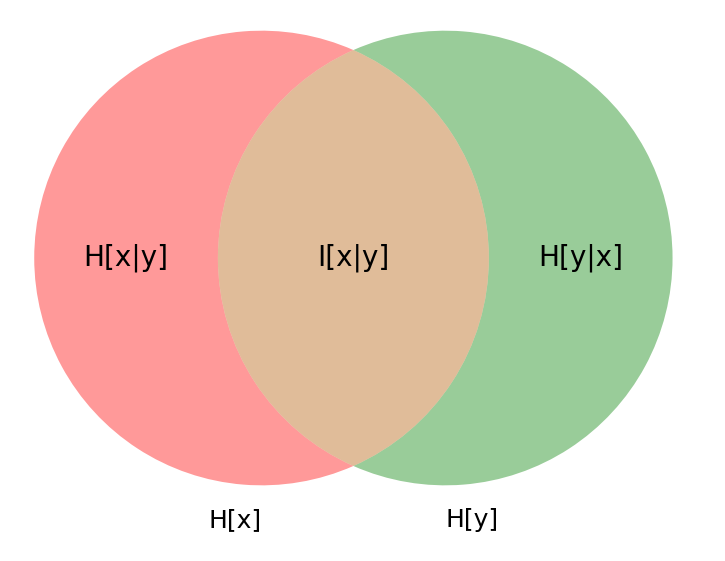
\includegraphics[width=0.8\linewidth]{diagram.png}
    \caption*{Exercise 1.39 Diagram}
\end{figure}
\end{proof}

\section*{Exercise 1.40 $\star$}
By applying Jensen's inequality $(\ref{eq:1.115})$ with $f(x) = \ln x$, show
that the arithmetic mean of a set of real numbers is never less than their
geometric mean.

\vspace{1em}

\begin{proof}
    Let $N$ be the cardinality of the considered set of real numbers. By considering
    $f(x) = \ln x$ (which is convex) and  $\lambda_i = 1/N$, we use Jensen's inequality
    to obtain:
    \begin{align*}
        \ln \bigg(\frac{1}{N} \sum_{i=1}^{N} x_i\bigg) 
        \leq \frac{1}{N} \sum_{i=1}^{N} \ln x_i
        = \frac{1}{N} \ln \bigg(\prod_{i = 1}^N x_i\bigg)
        = \ln \bigg\{\bigg(\prod_{i = 1}^N x_i\bigg)^{1/N}\bigg\}
    \end{align*}

    Since $\ln x$ is increasing, the above inequality is equivalent with:
     \[
         \frac{1}{N} \sum_{i=1}^{N} x_i \leq \bigg({\prod_{i = 1}^n x_i}\bigg)^{1/N}
    \] 
    which proves that the arithmetic mean of a set of real numbers 
    is never less than their geometric mean.
\end{proof}

\section*{Exercise 1.41 $\star$}
Using the sum and product rules of probability, show that the mutual
information $I(\mathbf{x}, \mathbf{y})$ satisfies the relation  $(\ref{eq:1.121})$.

\vspace{1em}

\begin{proof}
    The mutual information between the variables $\mathbf{x}$ and $\mathbf{y}$ is
    given by:
    \begin{equation}\label{eq:1.120}\tag{1.120}
        I[\mathbf{x}, \mathbf{y}] 
        = -\iint p(\mathbf{x}, \mathbf{y}) \ln \bigg(\frac{p(\mathbf{x})p(\mathbf{y})}
        {p(\mathbf{x}, \mathbf{y})}\bigg) \diff \mathbf{x} \diff \mathbf{y}
    \end{equation}

    We split the integral and use the product and sum rules of probability to obtain
    the desired result:
    \begin{align*}
        I[\mathbf{x}, \mathbf{y}] 
        &= -\iint p(\mathbf{x}, \mathbf{y}) \ln p(\mathbf{x}) \diff \mathbf{x} \diff \mathbf{y}
        + \iint p(\mathbf{x}, \mathbf{y}) \ln p(\mathbf{x} | \mathbf{y}) \diff \mathbf{x} \diff \mathbf{y} \\
        &= -\int p(\mathbf{x}) \ln p(\mathbf{x}) \diff \mathbf{x} 
        + \iint p(\mathbf{x}, \mathbf{y}) \ln p(\mathbf{x} | \mathbf{y}) \diff \mathbf{x} \diff \mathbf{y} \\
        &= H[\mathbf{x}] - H[\mathbf{x} | \mathbf{y}] \label{eq:1.121}\tag{1.121}
    \end{align*}

    Analogously, one could easily show that also
    $I[\mathbf{x}, \mathbf{y}] = H[\mathbf{y}] - H[\mathbf{y} | \mathbf{x}]$
\end{proof}
